% Intestazione
\fancyhead[L]{5 \hspace{0.2cm} Cruscotto di valutazione della qualità} % Testo a sinistra


\section{Cruscotto di valutazione della qualità}
\label{sec:Cruscotto di valutazione della qualità}


\subsection{Varianza dell'impegno orario}

\dots

\section*{Analisi}

\dots



\subsection{Varianza di budget}

\dots

\section*{Analisi}

\dots



\subsection{Estimate to Complete ed Estimate at Completion}

\dots

\section*{Analisi}

\dots



\subsection{Planned Value, Earned Value e Actual Cost}

\dots

\section*{Analisi}

\dots



\subsection{Schedule Variance e Cost Variance}

\dots

\section*{Analisi}

\dots



\subsection{Schedule Performance Index e Cost Performance Index}

\dots

\section*{Analisi}

\dots



\subsection{Misure di mitigazione insufficienti}

\dots

\section*{Analisi}

\dots



\subsection{Rischi inattesi}

\dots

\section*{Analisi}

\dots



\subsection{Requisiti soddisfatti}
\label{subsec:Requisiti soddisfatti}

\begin{figure}[h] 
    \centering
    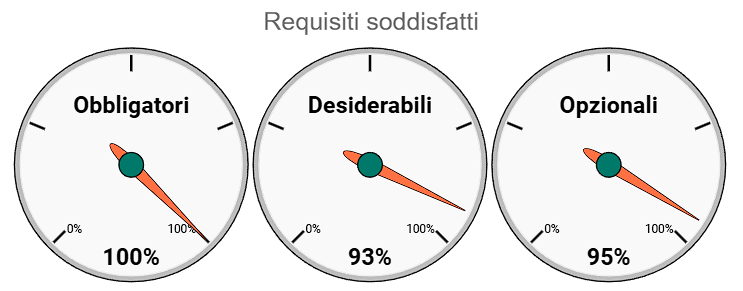
\includegraphics[width=\textwidth]{Requisiti soddisfatti.png}
    \caption{Requisiti obbligatori, desiderabili e opzionali soddisfatti} 
    \label{fig: Requisiti soddisfatti}
\end{figure}

\section*{Analisi}
Il progetto fino ad ora ha prodotto un Proof of Concept, dunque nessun prodotto finale con il quale soddisfare alcun requisito.
Per questo motivo è normale che nel cruscotto non risulti soddisfatto nessun requisito.



\subsection{Indice di Gulpease}

\dots

\section*{Analisi}

\dots